\documentclass{article}

\usepackage[utf8]{inputenc}
\usepackage[T1]{fontenc}
\usepackage[serbian]{babel}
\usepackage{amsmath}
\usepackage{amssymb}
\usepackage{tikz}
\usepackage{caption}
\usepackage{subcaption}
\usepackage{graphicx}

\title{Opis rada: Prekrivanje velikog broja tačaka kutijom male površine}
\author{Petar Nikić}
\date{\today}

\begin{document}

\maketitle

\section{O radu i autorima}

Rad \textbf{prekrivanje velikog broja tačaka kutijom male površine} (eng.~{\em Covering many points with a small area box})
objavljen je u časopisu {\em Journal of Computational Geometry} 10.07.2019. godine, pri čemu je inicijalna verzija podeljena
u decembru 2016. godine na sajtu arXiv. Autori rada su:

\begin{itemize}
	\item Mark de Berg, redovan profesor Tehnološkog univerziteta Ajndhoven u Holandiji i šef grupe za algoritme na unviverzitetu.
	Najveći doprinosi su mu u računarskoj geometriji. Napisao je dve knjige o računarskoj geometriji, pri čemu se jedna koristi kao
	opšteprihvaćen udžbenik za kurseve računarske geometrije.
	\item Sergio Cabello, redovan profesor Fakulteta matematike i fizike Univerziteta u Ljubljani. Glavna oblast istraživanja su
	mu algoritmi diskretne matematike.
	\item Otfried Cheong, profesor Računarskog fakulteta Korejskog naprednog instituta za nauku i tehnologiju. Njegova istraživačka
	grupa fokusirala se na diskretnu i računarsku geometriju.
	\item David Eppstein, odlikovan profesor katedre za računarstvo Univerziteta u Kaliforniji u Irvinu. Upravljao je centrom
	za algoritme i teoriju izračunljivosti, kao i centrom za algoritme, kombinatoriku i optimizaciju. Bavi se računarskom geometrijom
	i grafovskim algoritmima.
	\item Christian Knauer, profesor Instituta za primenjenu informatiku i vođa Grupe za algoritme i strukture podataka na Univerzitetu
	u Bajrojtu. Primarni fokus istraživanja mu je računarska geometrija.
\end{itemize}

\section{O problemima obrađenim u radu}

U radu autori opisuju dva usko vezana problema i predlažu dva algoritma koji se mogu koristiti za njihovo rešavanje.

\subsection{Opis problema}

Neka je $P$ skup od $n$ tačaka u ravni. U oba problema cilj je pokriti neki podskup tačaka \textbf{kutijom} (pravougaonikom sa ivicama koje su paralelne koordinatnim osama). U prvom problemu, ukoliko su dati $P$ i prirodni broj $k \geqslant 2$, traži se pravougaonik sa najmanjom površinom koji prekriva barem $k$ tačaka. U drugom problemu, za dat realan broj $\alpha > 0$, traži se najveći broj tačaka koji se može prekriti
kutijom površine ne veće od $\alpha$.

\subsection{Rezultati rada}

Za prvi problem, autori predlažu egzaktan algoritam kojim se pronalazi tražena kutija u složenosti $O \left( n k^2 \log n + n \log^2 n \right)$.
Za drugi problem, autori predlažu aproksimativan algoritam koji pronalazi kutiju koja {\em verovatno} pokriva $(1 - \varepsilon) \kappa^\ast$ tačaka,
gde je $\kappa^\ast$ maksimalan broj tačaka koje se mogu pokriti kutijom date površine. Algoritam je složenosti
$O \left( \frac{n}{\varepsilon^4} \log^3 n \log \frac{1}{\varepsilon} \right)$.

Autori posebno ističu da, ukoliko posmatramo $k$ i $\varepsilon$ kao konstante, dobijene složenosti algoritama su
$O (n \log^2 n)$ za prvi problem i $O (n \log^3 n)$ za drugi problem. Složenost ovih algoritama je znantno bolja u odnosu na prethodne algoritme koji rešavaju ovaj problem, u velikom broju slučajeva.

\subsection{Veza između problema}

Autori takođe ističu jaku vezu između ova dva problema. Ukoliko je površina za fiksirano $k$ manja od broja $\alpha$, onda se sa površinom $\alpha$ sigurno može pokriti barem $k$ tačaka, odnosno $k$ onda daje donju granicu za rešenje drugog problema za fiksirano $\alpha$.
Analogno, ukoliko je broj tačaka rešenja drugog problema veći od $k$ za neko fiksirano $\alpha$, površina rešenja prvog problema za $k$ je odozgo ograničena sa $\alpha$. Autori ističu da se algoritam koji predlažu za prvi problem može koristiti za određivanje rešenja drugog problema koristeći binarnu pretragu po rešenju.

\subsection{Raniji rezultati}

Konkretan problem pokrivanja $k$ tačaka kutijom najmanje površine razmatrali su Segal i Kedem, koji su opisali algoritam složenosti
$O ( n + k (n - k)^2 )$, koji je dobar kada je vrednost $k$ bliska vrednosti $n$. Opisani algoritam se može prilagoditi i problemu
pokrivanja $k$ tačaka kutijom {\em najmanjeg obima}, koji su obrađivali Aggarwal et al, Eppstein i Erickson, kao i Datta et al,
pri čemu se njihovi rezultati ne mogu proširiti na problem najmanje površine. Kaplan et al. su prikazali rešenje za problem minimalnog obima složenosti $O (n k^{3/2} \log k \log n)$, ali i minimalne površine složenosti $O (n^{5/2} \log^2 n)$.

Dva slična problema koja su takođe razmatrana su traženje najmanjeg diska koji sadrži barem $k$ tačaka, kao i traženje najmanjeg pravougaonika proizvoljne orijentacije koji sadrži barem $k$ tačaka.

\section{Algoritmi opisani u radu}

U nastavku su predstavljene osnovne ideje algoritama koje su autori predložili kao rešenje ranije pomenutih problema pokrivanja tačaka kutijom.

\subsection{Kutija najmanje površine koja pokriva barem $k$ tačaka}

Za rešenje prvog problema, autori rada predlažu tehniku podeli-pa-vladaj u kojoj skup tačaka dele na približno jednake skupove. Geometrijski,
tačke dele horizontalnom pravom, i onda rešavaju problem traženja najbolje kutije koja seče tu pravu razlaganjem na veći broj manjih problema.

Optimalno rešenje se traži između najboljeg rešenja za trenutnu pravu i rešenja dobijenih rekurzivnom primenom algoritma na podskupove
podeljene pravom. U nastavku stoji opis algoritma koji računa rešenje kada su dati skup tačaka $P$, traženi broj tačaka $k$ i prava $\ell$.

Za svaku tačku $p \in P$ i njoj simetričnu tačku $\bar{p}$ u odnosu na pravu $\ell$, algoritam generiše skup $Q_p$ na sledeći način:
izdvajaju se četiri dela ravni u prostoru između pravih paralelnih $\ell$ koje prolaze kroz $p$ i $\bar{p}$. Prvu podelu na dve ``ploče'' daje sama prava $\ell$, a drugu podelu daje prava koja povezuje $p$ i $\bar{p}$, čime se dobijaju četiri dela, $R_p^\leftarrow$, $R_p^\rightarrow$, $R_{\bar{p}}^\leftarrow$ i $R_{\bar{p}}^\rightarrow$, što se može videti na slici \ref{fig:regioni}.

Unutar svakog od delova, traži se do $k$ tačaka najbližih tačkama $p$ i $\bar{p}$ posebnim algoritmom, što nam daje skupove $P_p^\leftarrow$, $P_p^\rightarrow$, $P_{\bar{p}}^\leftarrow$ i $P_{\bar{p}}^\rightarrow$. Skupovi $Q_p$ se definišu kao unija navedenih skupova.

Za proizvoljan skup tačaka $Q$, tačku $q \in Q$ i broj $k$, autori uočavaju kutiju maksimalne površine koja sadrži bar $k$ tačaka iz $Q$ i koja sadrži tačku $q$ u gornjoj ili donjoj ivici kutije. Primer kandidata se može videti na slici \ref{fig:q-kutije}. Autori takođe opisuju algoritam koji se može koristiti za određivanje takve kutije.

\begin{figure}[h]
\centering
\begin{subfigure}[b]{0.45\textwidth}
\centering
\input{regioni.tkz}
\end{tikzpicture}
\caption{Prikaz podele ravni za tačku $p$ i pravu $\ell$.}
\label{fig:regioni}
\end{subfigure}
\hfill
\begin{subfigure}[b]{0.51\textwidth}
\centering
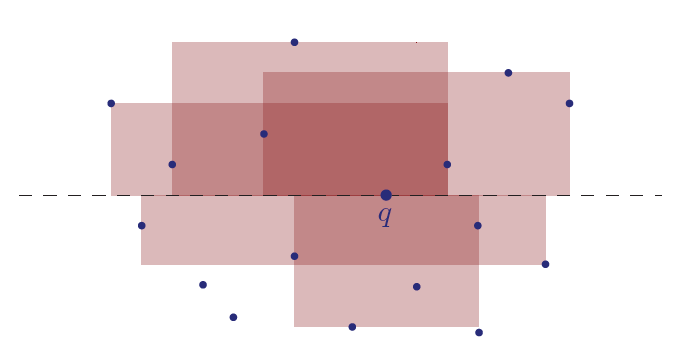
\includegraphics[width=\textwidth]{Q-kutije}
\caption{Prikaz razmatranih kutija gde je $q$ na donjoj ili gornjoj ivici za $k = 5$.}
\label{fig:q-kutije}
\end{subfigure}
\caption{Pojmovi u rešenju problema traženja kutije najmanje površine.}
\end{figure}

Generisanje podskupova $Q_p$ i uvođenje prethodnog koncepta opravdava dokazano tvrđenje autora da, ukoliko optimalna kutija za neko $k' \leqslant k$ seče pravu $\ell$, mora postojati $p_0 \in P$ takvo da kutija koju daje prethodni algoritam primenjen na $Q_{p_0}$, $p_0$ i $k'$ je takođe optimalna kutija. Intuitivno, optimalna kutija mora da ima neke tačke iz $P$ na gornjoj i donjoj ivici, $t^\ast$ i $b^\ast$. Može se pokazati da je optimalna kutija podskup $Q_{t^\ast}$ ili $Q_{b^\ast}$, zbog čega će algoritam, po definiciji, dati optimalno rešenje.

Primetimo da, pošto je $k' \leqslant k$ proizvoljno, možemo unapred da izračunamo skupove $Q_p$ i da ih koristimo za više upita. Ovaj pristup se koristi u aproksimativnom algoritmu koji rešava drugi problem, gde se vrši binarna pretraga po rešenju.

\subsection{Kutija date površine koja pokriva najviše tačaka}

Algoritam za približno određivanje kutije date površine koja pokriva najviše tačaka, koji autori predstavljaju, ima tri faze. Neka je $\kappa^\ast (P, \alpha)$ najveći broj tačaka koji pokriva kutija površine $\alpha$.

U prvoj fazi se traži prosta aproksimacija za $\kappa^\ast$, koja se razlikuje od optimalne vrednosti za konstantan faktor. Autori opisuju algoritam kojim se može dobiti vrednost $\kappa_a$ tako da važi:
\[ \frac{\kappa^\ast (P, \alpha)}{4} \leqslant \kappa_a \leqslant \kappa^\ast (P, \alpha). \] Primetimo takođe da onda važi
\[ \kappa^\ast (P, \alpha) \leqslant 4 \kappa_a \leqslant 4 \kappa^\ast (P, \alpha) ,\] tako da imamo i donju i gornju granicu za $\kappa^\ast$, $\kappa_a$ i $4 \kappa_a$.

Zatim, bira se uzorak $S$ tačaka iz $P$ veličine $s = \left\{ n, \frac{c}{\varepsilon^2}\frac{n}{\kappa} \log n \right\}$, pri čemu je $\kappa = 4 \kappa_a$, a $c$ neka prikladna konstanta. Autori su dokazali da, ukoliko se uzorak bira na ovakav način, važi da za svaku kutiju $R$ takvu da joj je površina manja od $\alpha$ važi \[\left|\frac{\left|P \cap R\right|}{n} - \frac{\left|S \cap R\right|}{s}\right| \leqslant \varepsilon \cdot \frac{\kappa}{n}\]
sa verovatnoćom $1 - \frac{1}{n}$.

U finalnoj fazi, koristi se aproksimacija $4 \kappa_a$ kao vrednost $k$ za generisanje svih skupova $Q_p$ pomenutih u opisu prvog problema, pri čemu se ne koristi skup $P$, već uzorak $S$. Zatim, pošto znamo da je vrednost $\kappa^\ast \in \left[ \kappa_a, 4 \kappa_a \right]$, u tom intervalu (u koracima $\varepsilon \kappa_a$) se vrši binarna pretraga gde se rešava prvi problem za $S$ i trenutnu vrednost pretrage i traži se prelazna tačka u kojoj minimalna površina postaje veća od $\alpha$, pri čemu je rezultat algoritma kutija koja se dobija na prelaznoj tački, površine manje od $\alpha$.

Algebarski se može pokazati da binarna pretraga daje rešenje koje pokriva makar $(1 - \varepsilon) \kappa^\ast (S, \alpha)$ tačaka, kao i da, na osnovu karakteristika uzorka, rešenje pokriva makar $(1 - 9 \varepsilon) \kappa^\ast (P, \alpha)$. Smenom $\varepsilon' = \varepsilon / 9$, dobija se željeni rezultat.

\end{document}